\subsection{Snorken}\label{section:snorken}
Snorken er et åbenlyst faktor, der skal tages højde for når man skal opdage søvn ved hjælp af sensorer, idet at en af de primære sensorer, som bruges til at bestemme om en person sover er lyd.
Hvis lyden gentagne gange optager snorken, vil den nuværende sandsynlighedsudregningen for denne sensor falde hver eneste gang snorken bliver optaget, og dette er helt klart et problem, som skal arbejdes videre på.

Et eksempel kan ses i \cref{fig:snorke-vs-ikkesnorken} hvor vi sammenligner en person som vi ved snorker mod en som ikke snorker.

\begin{figure}[h]
\begin{subfigure}{0.49\textwidth}
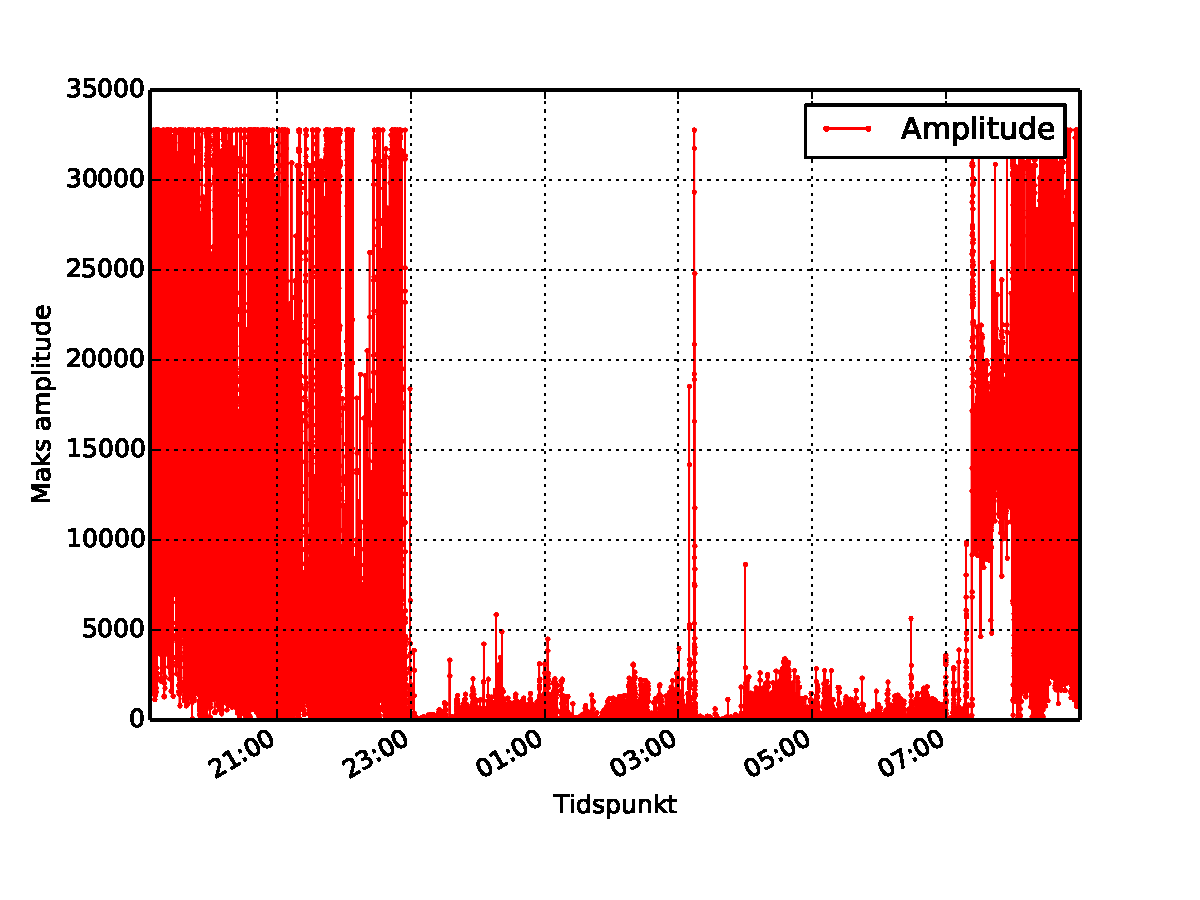
\includegraphics[width=1\textwidth,trim = 0cm 1cm 1cm 1cm,clip]{amplitude-plot-snorken}
\caption{Person der snorker}
\label{fig:person-snorker}
\end{subfigure}
\begin{subfigure}{0.49\textwidth}
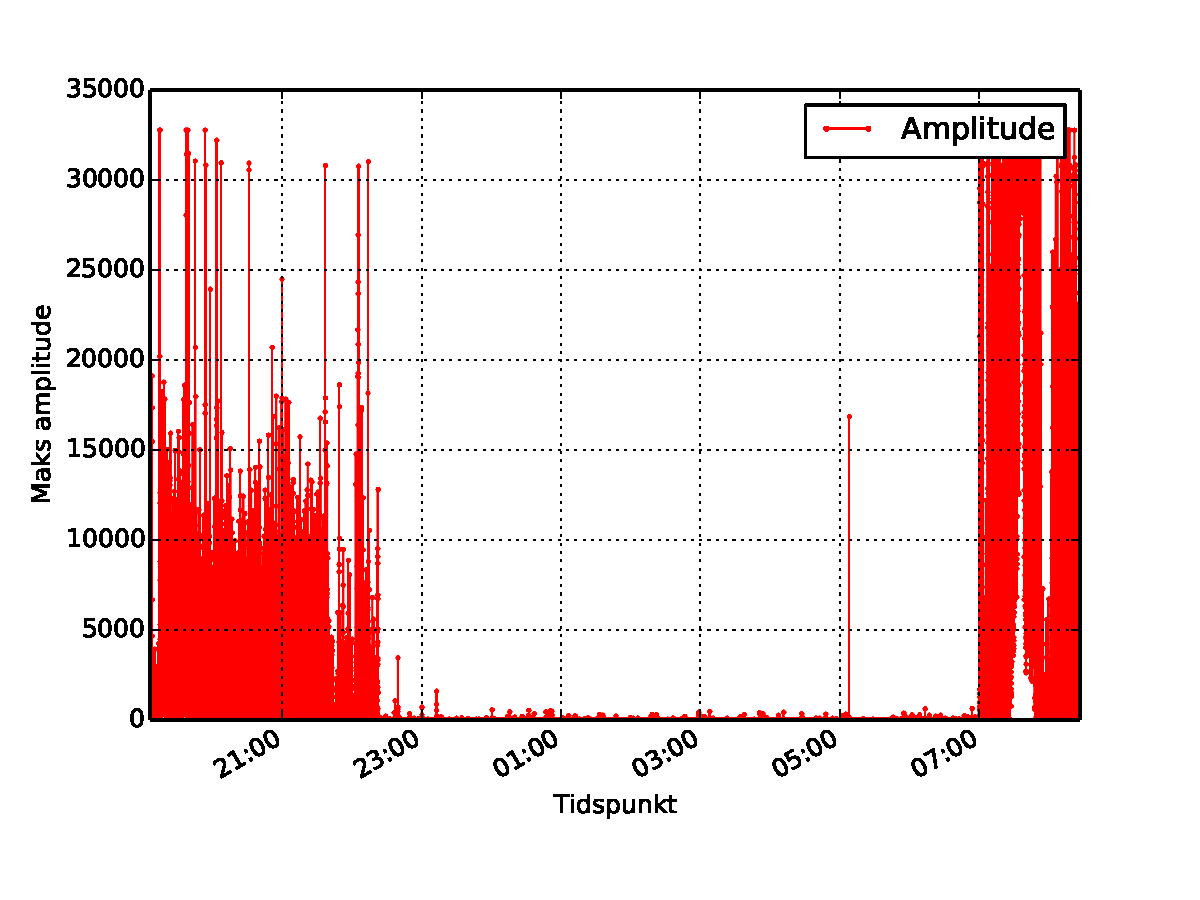
\includegraphics[width=1\textwidth,trim = 0cm 1cm 1cm 1cm,clip]{amplitude-plot-ingen-snorken}
\caption{Person der ikke snorker}
\label{fig:person-ikke-snorker}
\end{subfigure}
\caption{Person vi ved snorker og person vi ved ikke snorker}
\label{fig:snorke-vs-ikkesnorken}
\end{figure}

Hvis man ser på grafen med snorken, \cref{fig:person-snorker}, kan man se at amplituden er mere irregulær i søvn perioden i forhold til grafen i \cref{fig:person-ikke-snorker}. 
En simpel løsning på hvordan man kunne ignorere snorken i sandsynlighedsestimeringen vil være at sætte amplitude tærskelværdi op på et højere niveau, hvilket baseret på graferne kan være 5000. 
Tærskelværdien er den amplitude hvor den betragtes som ligegyldig idet at den ikke er høj nok, og kan derfor ses som et 0 når sandsynligheden udregnes. 
Men dette skal være baseret på hvor højt personen snorker og skal derfor være dynamisk, hvilket kan gøre at denne løsning ikke er optimal. 
Derudover, kan man ikke garantere at der ikke findes personer, der snorker lige så højt som når de snakker.
Andre metoder på at registrere søvn er derfor undersøgt.

Ud fra artiklerne \citet{Dafna2013}, \citet{Calabrese20111101} og \citet{7051338} dannes der et grundlag for hvordan snorken kan registreres.

\citet{Dafna2013} gør brug af et system til at inddele snorken og andre akustiske hændelser gennem et søvnforløb ved brug af lyd data, der blev optaget med en mikrofon ved en polysomnigrafisk undersøgelse. 
De endte med et meget præcist system, som kunne adskille snorken og andre akustiske hændelser med ~98\% nøjagtighed.
Denne metode kan tilpasses ind i vores system på den måde, at hvis snorken kan opdages har den ikke en negativ indflydelse, men derimod have en positiv indflydelse på sandsynlighedsberegningen af søvn. 
De bruger lyd data og ikke bare amplituden, så det vil være nødvendigt at undersøge om systemet også kan fungere ved brug af amplitude.

\citet{Calabrese20111101} forslår et system, der skal bruges til diagnosticering af søvnapnø ved hjælp af optaget lyd.
Dog blev der kun implementeret en prototype af systemet og den er derfor ikke blevet evalueret ordenligt endnu. 
Idéen er at man bruger analyser såsom 'Fast Fourier Transform' og 'Power Spectrum' til at finde tidspunkter, hvor personen har snorket baseret på optaget lyd. 
Denne metode sår tvivl ved løsningen om blot at indsamle maks amplitude, da om nødvendigt skal lydindsamlingen ændres til et sliding window.
Det vil sige, hvor vi samler det rå lyddata fra mikrofonen, men sletter lyddate efter en analyse er foretaget, således at privatlivs kriteriet stadig opfyldes.
Dette er en mulighed et modul kan benytte sig af, og bør udforskes med videre arbejde.

\citet{7051338} udvikler et system, der kan registrer snorken ud fra lydoptagelser.
Denne metode bruger machine learning til at udvikle en model der detektere hvornår folk sover.
Metoden der er udviklet gør brug af en \textit{K}-Nearest Neighbour classifier.
Derudover, kræver metoden ligesom den forrige at vi optager lyd i stedet for bare at se på amplituden.
I modsætning til \citet{Calabrese20111101}, fokuseres der på at registre snorken, hvilket også kvalificerer denne metode som en oplagt kandidat til videre udforskning.

Hvis man vælger at arbejde videre med en af disse metoder til at detektere snorken, har det også andre anvendelsesmuligheder end at fjerne støj fra vores estimering.
Hvis en af metoderne registrerer at man snorker, kan man sige at det uden tvivl betyder at en person sover, og så kan den procentvurdering der ellers havde været på det tidspunkt blive overskrevet med 100\%.
Dette er en meget relevant ting at bruge snorke registrering til, da det vil forbedre nøjagtigheden meget, i stedet for bare at fjerne støj.
